\documentclass[tikz,border=5pt]{standalone}
\usepackage{amsmath,amssymb}
\usepackage{tikz}
\begin{document}
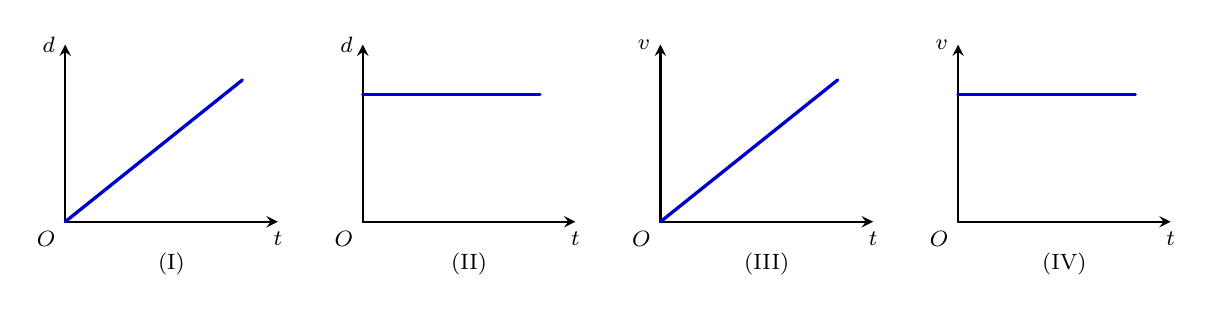
\begin{tikzpicture}[>=stealth, line join=round, line cap=round, font=\footnotesize, scale=0.9]
	% ĐỒ THỊ (I): d - t thẳng qua gốc O
	\begin{scope}[shift={(0,0)}]
		\draw[->, thick] (0,0) -- (3,0) node[below] {$t$};
		\draw[->, thick] (0,0) -- (0,2.5) node[left] {$d$};
		\draw[very thick, blue!80!black] (0,0) -- (2.5,2);
		\node[below left] at (0,0) {$O$};
		\node at (1.5,-0.6) {(I)};
	\end{scope}
	
	% ĐỒ THỊ (II): d - t nằm ngang
	\begin{scope}[shift={(4.2,0)}]
		\draw[->, thick] (0,0) -- (3,0) node[below] {$t$};
		\draw[->, thick] (0,0) -- (0,2.5) node[left] {$d$};
		\draw[very thick, blue!80!black] (0,1.8) -- (2.5,1.8);
		\node[below left] at (0,0) {$O$};
		\node at (1.5,-0.6) {(II)};
	\end{scope}
	
	% ĐỒ THỊ (III): v - t thẳng qua gốc O
	\begin{scope}[shift={(8.4,0)}]
		\draw[->, thick] (0,0) -- (3,0) node[below] {$t$};
		\draw[->, thick] (0,0) -- (0,2.5) node[left] {$v$};
		\draw[very thick, blue!80!black] (0,0) -- (2.5,2);
		\node[below left] at (0,0) {$O$};
		\node at (1.5,-0.6) {(III)};
	\end{scope}
	
	% ĐỒ THỊ (IV): v - t nằm ngang
	\begin{scope}[shift={(12.6,0)}]
		\draw[->, thick] (0,0) -- (3,0) node[below] {$t$};
		\draw[->, thick] (0,0) -- (0,2.5) node[left] {$v$};
		\draw[very thick, blue!80!black] (0,1.8) -- (2.5,1.8);
		\node[below left] at (0,0) {$O$};
		\node at (1.5,-0.6) {(IV)};
	\end{scope}
\end{tikzpicture}
\end{document}
